\documentclass[a4paper,12pt]{article} 
\usepackage{geometry}
\geometry{
	a4paper,
	total={170mm,257mm},
	left=20mm,
	top=20mm,
}
\usepackage{titlesec}
\titlelabel{\thetitle.\quad} %точка в section

%%% Работа с русским языком
\usepackage{cmap}                           % поиск в PDF
\usepackage{mathtext} 			 	       % русские буквы в формулах
\usepackage[T2A]{fontenc}               % кодировка
\usepackage[utf8]{inputenc}              % кодировка исходного текста
\usepackage[english,russian]{babel}  % локализация и переносы

%Математика
\usepackage{amsmath,amsfonts,amssymb,amsthm,mathtools} % AMS
\usepackage{icomma} % "Умная" запятая

%% Шрифты
\usepackage{euscript}	 % Шрифт Евклид
\usepackage{mathrsfs} % Красивый матшрифт

%% Команды
\DeclareMathOperator{\const}{\mathop{const}}

%% Перенос знаков в формулах
%\newcommand*{\hm}[1]{#1\nobreak\discretionary{}
%	{\hbox{$\mathsurround=0pt #1$}}{}}

%%% Заголовок
\author{Шерхалов Денис Б02-204}
\title{Лабораторная работа 2.1.2 \\
	\textbf{Определение $C_p / C_v$ методом изобарического расширения}}
\date{\today}

\begin{document}
	
	{\Large \maketitle}
	
	\subparagraph*{Цель работы:}определение отношения $C_p / C_v$ воздуха по измерения давления в стеклянном сосуде. Измерения проводятся сначала после адиабатического расширения газа, а затем после изохорического нагревания сосуда и газа до комнатной температуры.

	\subparagraph*{В работе используются:}стеклянный сосуд: U-образный жидкостный манометр; резиновая груша; газгольдер с воздухом, секундомер. 
	
	\subparagraph*{Экспериментальная установка.} Экспериментальная установка состоит из стеклянного сосуда А (объёмом около 20 л), снабжённого краном $К$, и U-образного жидкостного манометра, измеряющего избыточное давление газа в сосуде. Схема установки показана на Рис. 1. 

	\begin{figure}[h!]
		\centering{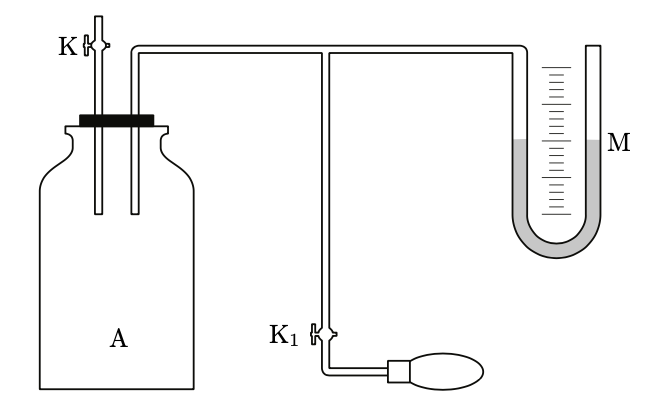
\includegraphics[width=0.5\textwidth]{1.jpg}}
		\caption[]{\label{fig:1} Установка для определения $C_p / C_v$ методом адиабатического расширения газа}
	\end{figure}


	\section{Введение} Избыточное давление создаётся с помощью резиновой груши, соединённой с сосудом трубкой с краном $К_1$, в сосуде создаётся заданное избыточное давление $p_1$. При этом газ становится перегретым.
	
	Мысленно выделим в сосуде некоторый объём $\Delta V$. Будем следить за изменением его состояния. Вследствие теплообмена со стенками сосуда через некоторое время газ остынет до комнатной температуры $T_0$ (изохорное охлаждение). При этом давление понизится до $p_0 + \Delta p_1$, где
\begin{equation*}
	\Delta p_1 = \rho g \Delta h_1
	\eqno(1)
\end{equation*}
	
	Откроем кран $K_1$. За время $\Delta t$ порядка $0.5с$ произойдёт адиабатическое расширение газа, и его температура окажется ниже комнатной. Далее газ будет изобарически нагреваться. Зададим время $\tau$, В течение которого кран $K$ остаётся открытым, таким, чтобы можно было пренебречь временем $\Delta t$ адиабатического расширения воздуха. После закрытия крана $K$ газ станет изохорически нагреваться до комнатной температуры, причём давление внутри сосуда возрастёт до $p_0 + \Delta p_2$, где
	\begin{equation*}
		\Delta p_2 = \rho g \Delta h_2
		\eqno(2)
	\end{equation*}

	Наибольший интерес представляет исследование зависимости отношения перепадов давления $\dfrac{\Delta p_1}{\Delta p_2}$ от времени $\tau$.
	
	С хорошей точностью мы можем считать воздух в газгольдере идеальным газом. Рассмотрим изобарическое расширение воздуха. Для этого запишем уравнение теплового баланса для изменяющейся со временем массы $m = \dfrac{p_0 V_0}{RT}\mu$:
	\begin{equation*}
		c_p \, m \, dT = -\alpha (T - T_0)dt
	\end{equation*}
	где $c_p$ -- удельная теплоёмкость воздуха при постоянном давлении, $\alpha$ -- положительный постоянный коэффициент, характеризующий теплообмен, $V_0$ -- объём газгольдера.
	\begin{gather*}
		\dfrac{dT}{T(T - T_0)} = \dfrac{-\alpha dt}{c_p \,\dfrac{p_0 V_0}{R}\mu} 
		\quad \Rightarrow \quad 
		\dfrac{1}{T_0}\left(\dfrac{1}{T} - \dfrac{1}{T - T_0}\right) dT = \dfrac{\alpha dt}{c_p m_0 T_0} 
		\quad \Rightarrow \\ \Rightarrow \quad 
		\int_{T_1}^{T_2}\left(\dfrac{1}{T} - \dfrac{1}{T - T_0}\right) dT = \dfrac{\alpha}{c_p m_0}\int_{0}^{\tau}dt 
		\quad \Rightarrow \quad 
		\ln\left(\dfrac{T_2}{T_1}\right) - \ln\left(\dfrac{T_2 - T_0}{T_1 - T_0}\right) = \dfrac{\alpha}{c_p m_0}\tau 
		\quad \Rightarrow \\ \qquad\qquad\qquad\Rightarrow \quad
		\ln\left(\dfrac{T_2}{T_1}\dfrac{\Delta T_1}{\Delta T_2}\right) = \dfrac{\alpha}{c_p m_0}\tau 
		\quad \Rightarrow \quad 
		\dfrac{\Delta T_1}{T_1} = \dfrac{\Delta T_2}{T_2} \exp\left(\dfrac{\alpha}{c_p m_0}\tau\right)
		\qquad \qquad \qquad(3)
	\end{gather*}
	Для адиабатического расширение справедливо соотношение $T^{\gamma} = \const\, p^{\gamma - 1}$, где $\gamma = \dfrac{c_p}{c_v}$
	
	\begin{equation*}
		\gamma\dfrac{dT}{T} = (\gamma - 1)\dfrac{dp}{p} 
		\quad \Rightarrow \quad 
		\dfrac{dT}{T} = \dfrac{(\gamma - 1)}{\gamma}\dfrac{dp}{p} 
		\quad \Rightarrow \quad 
		\dfrac{\Delta T_1}{T_1} = \dfrac{(\gamma - 1)}{\gamma}\dfrac{dp_1}{p_0} 
		\eqno(4)
	\end{equation*}
	При изохорическом нагреве газа выполняется соотношение: 	
	\begin{equation*}
		\dfrac{p}{T} = \const \quad \Rightarrow \quad \dfrac{dp}{p} = \dfrac{dT}{T} \quad \Rightarrow \quad \dfrac{\Delta p_2}{p_0} = \dfrac{\Delta T_2}{T_2}
		\eqno(5)
	\end{equation*}
	После подстановки (4) и (5) в (3) получим:
	\begin{gather*}
		\dfrac{(\gamma - 1)}{\gamma}\dfrac{\Delta p_1}{p_0} = \dfrac{\Delta p_2}{p_0}\exp\left(\dfrac{\alpha}{c_p m_0}\tau\right)
		\quad \Rightarrow \quad
		\dfrac{(\gamma - 1)}{\gamma}\Delta h_1 = \Delta h_2\, \exp\left(\dfrac{\alpha}{c_p m_0}\tau\right)
		\quad \Rightarrow \\ \qquad \Rightarrow \quad 
		\dfrac{\Delta h_1}{\Delta h_2} = \dfrac{\gamma}{\gamma - 1}\exp\left(\dfrac{\alpha}{c_p  m_0}\tau\right)
		\quad \Rightarrow \quad 
		\ln\left(\dfrac{\Delta h_1}{\Delta h_2}\right) = \ln\left(\dfrac{\gamma}{\gamma - 1}\right) + \left(\dfrac{\alpha}{c_p  m_0}\right)\tau \qquad \qquad (6)
	\end{gather*}
	
	
	\section{Выполнение}
	
	\subparagraph*{1.} Проверим исправность установки. Убедимся, что уровни жидкости в манометре одинаковы. Закачаем с помощью груши газ и подождём выравнивания температур. Запишем разность уровней жидкости $\Delta h_1$. Откроем кран К на короткое время ($\tau \approx 0,5c$) и закроем его снова. Подождём, пока уровень жидкости в манометре перестанет изменяться, т.е. когда температура газа в сосуде сравняется с комнатной. Запишем разность уровней жидкости в манометре $\Delta h_2$. Далее проведём серию из 6 измерений сначала для других времён открытия крана $\tau$. По полученным данным построим график зависимости $\ln\left(\dfrac{\Delta h_1}{\Delta h_2}\right)$ от $\tau$ (График №1), а далее найдём из него $\gamma$ используя формулу (6).
	
	\subparagraph*{2.} Рассчитаем погрешность для графика: $$\Delta \tau = \pm0,5 с, \qquad \Delta\left(\ln\left(\dfrac{\Delta h_1}{\Delta h_2}\right)\right) = \pm2\,\delta h\dfrac{\Delta h_2}{\Delta h_1}$$
	\begin{table}[h!] 
		\caption{Результаты эксперимента,$\;$ $\Delta \tau = \pm0,5 с,\;\; \delta h = \pm0,1 см$}
		\begin{center}
			\begin{tabular}{|*{4}{l|}}
				\hline
				№ & $\tau$, c & $\Delta h_1$, см & $\Delta h_2$, см\\ \hline
				1 & 0,5 & 16.0 & 4.4 \\ \hline
				2 & 5 & 15.3 & 3.4 \\ \hline
				3 & 10 & 13.2 & 2.4 \\ \hline
				4 & 15 & 12.3 & 1.8 \\ \hline
				5 & 20 & 12.0 & 1.4 \\ \hline 
				6 & 25 & 12.6 & 1.2 \\ \hline
				7 & 30 & 12.1 & 0.9 \\ \hline 
			\end{tabular}
		\end{center}
	\end{table}
	
	\begin{figure}[h!]
		\centering{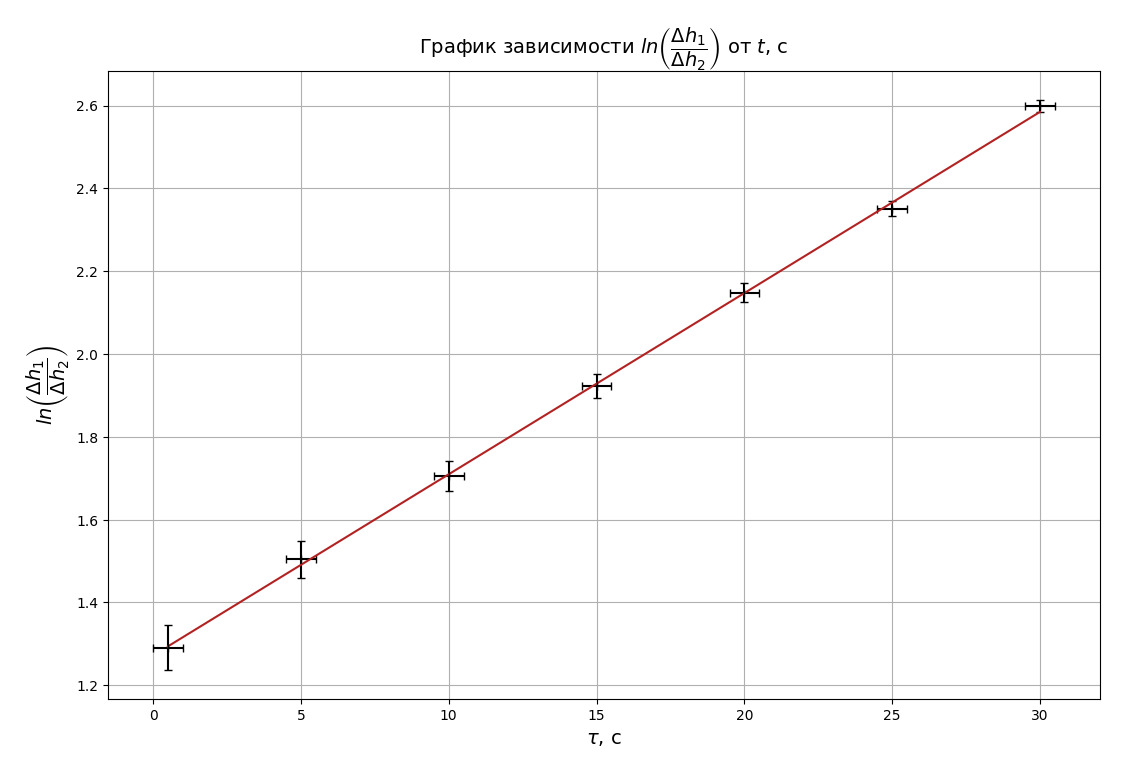
\includegraphics[width=1\textwidth]{graph1.png}}
		\caption[]{\label{fig:2} График №1}
	\end{figure}

	Используя библиотеки $NumPy$ и $Matplotlib$ на $Python$ построим график по МНК и получим погрешность. 
	\begin{equation*}
		b = \ln\left(\dfrac{\gamma}{\gamma - 1}\right) = 1.272 \pm 0.041\quad \Rightarrow \quad \sigma_b = 3.22\% 
	\end{equation*}
	Далее найдем $\gamma$. Приравняем $\sigma_b = \sigma_{\gamma} \approx 3.22\%$ 
	\begin{equation*}
		\gamma = \dfrac{e^b}{e^b - 1} = 1.389 \pm 0.045
	\end{equation*}


	\section{Вывод}
	
	В ходе эксперимента при использовании знаний полученных в ходе курса термодинамики было получено значение показателя адиабаты для воздуха. Полученное значение \\
	$\gamma = \dfrac{c_p}{c_v} = 1.389 \pm 0.045$ в пределах погрешности ($\sigma_{\gamma} = 3.22\%$) совпало с табличным \\ $\gamma^* = 1.4$. Неполное совпадение результата вызвано, во-первых, погрешностью в определении времени $\tau$, а во-вторых с тем, что снятая мной разница уровней воды в трубке не всегда была окончательной, т.к. установление идеального равновесия требует слишком большого времени ожидания.
	
\end{document}